
\documentclass[spanish]{article}% use option titlepage to get the title on a page of its own.
\usepackage{cite}
\usepackage{listings}
\usepackage{color}
\usepackage{graphicx}
\usepackage{enumitem}
\usepackage{float}

\usepackage[T1]{fontenc}
\usepackage{selinput}
\SelectInputMappings{%
  aacute={�},
  ntilde={�},
  Euro={�}
}
\usepackage{babel}




\definecolor{dkgreen}{rgb}{0,0.6,0}
\definecolor{gray}{rgb}{0.5,0.5,0.5}
\definecolor{mauve}{rgb}{0.58,0,0.82}

\lstset{frame=tb,
  language=Python,
  aboveskip=3mm,
  belowskip=3mm,
  showstringspaces=false,
  columns=flexible,
  basicstyle={\small\ttfamily},
  numbers=none,
  numberstyle=\tiny\color{gray},
  keywordstyle=\color{blue},
  commentstyle=\color{dkgreen},
  stringstyle=\color{mauve},
  breaklines=true,
  breakatwhitespace=true,
  tabsize=3
}
\begin{document}

\begin{titlepage}
	\begin{center}
	\line(1,0) {300} \\
	\huge{\textbf{Optimizaci�n de Flujo en Redes: Reporte 4 }}
	\line(1,0) {300}\\
	
	\textsc{ \Large Mayra Cristina Berrones Reyes.  6291}\\ 
	\textsc{\Large Abril 2018} \\
	\end{center}
\end{titlepage}

\section*{Introducci�n}

Para este reporte se estar�n utilizando tanto nuevos conceptos, como los que ya se hab�an implementado en reportes anteriores. Por ejemplo, en caso de nuevos conceptos, se estar�n dando a conocer temas como clustering (tambi�n conocido como agrupamiento) es una de las t�cnicas de miner�a de datos el cual consiste en la divisi�n de los datos en grupos de objetos similares. Cuando se representan la informaci�n obtenida a trav�s de clusters o racimos se pierden algunos detalles de los datos, pero a la vez se simplifica dicha informaci�n. \cite{clus}
\\

En este caso, hablaremos de agrupamientos en relaci�n con los grafos que se han estado realizando a lo largo del semestre.
\\

El segundo concepto que estaremos visitando, es de la densidad de nuestro grafo. Esto lo iremos desarrollando a lo largo de este trabajo, bas�ndonos en el n�mero de aristas que conectan a los nodos, as� como de algunos c�lculos de promedios que se explicar�n mas adelante.

\section*{Modificaci�n del grafo principal}

Primeramente, iniciamos con una nueva forma del grafo. Ya no simplemente hacemos que los nodos se acomoden de manera aleatoria a lo ancho y largo del plano, si no que se les da un acomodo circular para poder apreciar mejor las conexiones que se tienen entre ellos y poder hacer un an�lisis mas a fondo de el porque de estas conexiones.
\\
La forma circular de los nodos se logr� gracias al siguiente extracto de c�digo, que se tom� del archivo intento.py.


\begin{lstlisting}
	def puntos (self, num, k):
		self.n = num
		self.k = k
		
		th = 2*(pi)/self.n
		with open ("grafica.dat", 'w') as salida:
			for i in range(self.n):
				x = sin(th*i)
				y = cos(th*i)
				self.P.append((x, y, i))
				self.nodos.append((x,y))
				if not (x, y) in self.vecinos:
					self.vecinos[(x,y)] = []
				print (x, y, i, file = salida)
\end{lstlisting}

A grandes rasgos, lo que queremos recalcar aqu�, es el hecho de que se utilizaron las funciones de la librer�a de MATH de Python para poder utilizar las funciones del seno y coseno, lo que facilito mucho mas poder posicionar los nodos en su forma circular.


\begin{figure*}[h!] 
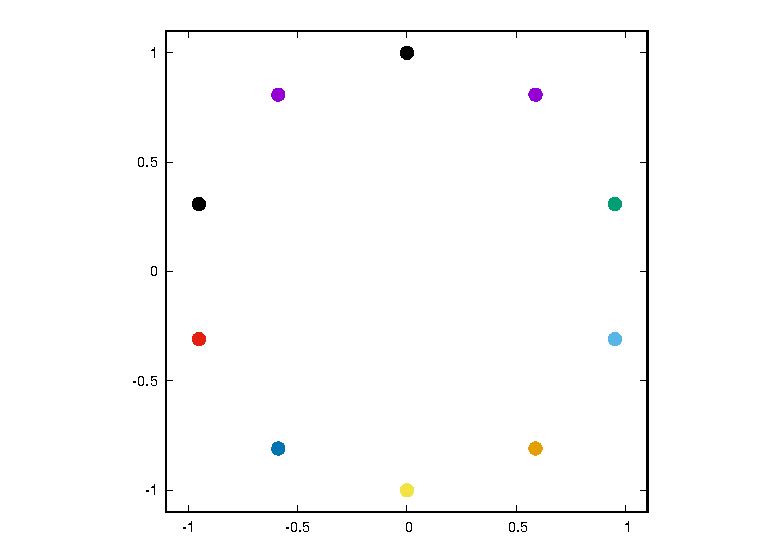
\includegraphics[width = 1\textwidth]{circulo.eps}
\caption{Nodos acomodados de manera circular dentro del plano.}
\label{td}
\end{figure*}


\section*{Conexiones principales y secundarias}

Antes de iniciar con los conceptos de agrupamiento y densidad que se mencionaban al inicio de este reporte, para realizar las conexiones de los nodos se realizara una variaci�n de lo que se hacia en reportes anteriores. Por ejemplo, en el reporte 3() se tomaba una probabilidad al azar gracias a un numero que se le asignaba con la herramienta Random() de Python, y dependiendo de este numero aleatorio, era la cantidad de aristas que estar�an asignadas a cada nodo.

En dicho reporte, tambi�n manej�bamos direcciones y pesos. Esto se deja un poco de lado en este reporte. Lo que rescatamos de aqu� un poco, es la forma de unir los nodos.
Primeramente, tomaremos un valor K, el cual se tiene que asignar un valor mas bajo que la mitad de los nodos totales por el siguiente motivo. El objetivo de esta variable K es juntar a un nodo con su k- esimo vecino por ambos lados. Si tenemos, por ejemplo, un grafo de 10 nodos, y queremos darle una k de 6, esto seria redundante, ya que ya existir�a una arista que esta uniendo a los �ltimos nodos que se quisieran emparejar.



\begin{thebibliography}{X}
\bibitem{reporte} \textsc{Berrones Reyes, Mayra Cristina} \textit{Reporte3. Marzo 2018}
\bibitem{elisa} \textsc{Schaeffer, Elisa} \textit{https://elisa.dyndns-web.com/teaching/mat/discretas/md.html} \textsc{Matem\'aticas Discretas. Grafos y \'arboles.}  \textbf{Consultado en Abril 2018}
\bibitem{clus} \textsc{Clustering} \textit{ECURed, https://www.ecured.cu/Clustering} \textbf{Consultado en Abril 2018}


\end{thebibliography}

\end{document} 












